%!TEX root = ../../dissertation.tex
%%%%%%%%%%%%%%%%%%%%%%%%%%%%%%%%%%%%%%%%%%%%%%%%%%%%%%%%%%%%%%%%%%%%%%%%%%%%%%%%
\section{Mobile Reliable Streaming Simulations}
\label{c6:sec:mobilestreamingtestbed}

However, some experiments can not be easily conducted in active measurement testbeds, for example due to the necessary scale to achieve meaningful results. Especially, new protocols or adaptations to existing ones are preferentially first tested in a network simulation. Simulation frameworks are especially important for mobile networks, as acquiring packet-level traces and information about every node in an actual commercially operating cellular network is nigh impossible due to the users' privacy and the provider's business concerns.

While there are some active measurement studies specifically targeted at reliable streaming in mobile networks, e.g., \cite{Muller:2012:EDA:2151677.2151686}, most are conducted either in fixed networks or using simulation frameworks. Therefore, to better evaluate reliable streaming, it would be very desirable to find an existing framework, that covers all important aspect in 3G or 4G mobile networks.

There are a number of network simulators readily available for use, both commercial as well as \gls{FOSS}. But only a small subset of them has the capability (or can be extended) to simulate \gls{3G} or LTE networks. Even further, most radio network capable simulators only concern themselves with the physical radio link and completely neglect all other network paths, especially the core and all control plane signaling interactions. 

The following list overviews current publicly available simulation frameworks with \gls{3G}/\gls{LTE} support:

\begin{itemize}
	\item An external \gls{UMTS} module\footnote{\url{http://net.infocom.uniroma1.it/reti_files/reti_downloads.htm}} is available for the no longer maintained \textbf{ns-2} simulation framework. A further separate collection of patches\footnote{\url{http://seacorn.cs.ucy.ac.cy/eumtssim/}} also extends ns-2 with \gls{UMTS} radio link capabilities~\cite{vranjevs2011use} but it is not publicly available.

	Both are as of August 2014 no longer being developed and not up-to-date to the newest specifications. They also focus solely on the user plane radio physical and link layer of \gls{UMTS}.

	\item Another third-party radio link layer simulation model is available for \textbf{MATLAB}\footnote{\url{http://www.nt.tuwien.ac.at/research/mobile-communications/lte-simulators/}}~\cite{mehlfuhrer2011vienna}.

	\item A standalone \gls{LTE} simulation\footnote{\url{http://telematics.poliba.it/index.php/en/lte-sim}}~\cite{5634134} includes models for some \gls{LTE} nodes, including the \gls{eNB} and \gls{MME} and implements a selection of protocols (\gls{PDCP}, \gls{RLC}, and \gls{RRC}).

	However, the implementation of these nodes and protocols is rudimentary at best and is not even close to the actual specification. Additionally, the simulator lacks a \gls{TCP}/\gls{IP} stack as \gls{IP} is reduced to its basic functionality and \gls{TCP} is completely absent.

	\item A framework dubbed SimuLTE\footnote{\url{https://github.com/inet-framework/simulte}} is available for \textbf{OMNeT++}\footnote{\url{http://www.omnetpp.org/}}. Included are the user plane aspects of the radio link and some basic \gls{SGW} and \gls{PGW} functionality.

	\item The \textbf{ns-3}\footnote{\url{http://www.nsnam.org}} simulator already contains an \gls{LTE}/\gls{EPC} module called LENA\footnote{\url{http://networks.cttc.es/mobile-networks/software-tools/lena/}}~\cite{Baldo:2013:OSM:2507924.2507940} with features similar to SimuLTE. Again, only user plane \gls{SGW}/\gls{PGW} functionality is present with an initial \gls{GTP-U} implementation.
\end{itemize}

The goal here is to simulate reliable streaming in a realistic mobile environment. That includes both a complete horizontal network path --- both the radio link as well as the core network --- as well as a vertical network stack --- comprising both user plane and control plane.

Unfortunately, none of the above feature a complete representation, which can be at least partially attributed to the complexity of the \gls{3GPP} specifications. Nonetheless, the simulators could still provide a viable basis for a mobile streaming framework while keeping the limitations in mind.Between these a decision needs to be made as to the basis of the mobile streaming simulation framework. 

Ultimately, the choice fell on ns-3 with the LENA module. Alongside with SimuLTE it has the most complete \gls{LTE} representation. And targeting \gls{LTE} networks seems to be the more future-proof path in the the long term. With the exception of OMNeT++, which has comparable capabilities, ns-3's \gls{TCP}/\gls{IP} is much more complete and realistic than that of the other frameworks. Additionally, it can also incorporate the actual \gls{TCP}/\gls{IP} of older Linux kernels with NSC\footnote{\url{http://research.wand.net.nz/software/nsc.php}}. As an additional feature, ns-3 can also act as a network emulator for real network traffic. This will be exploited in the upcoming model.

In the long run, to better represent actual mobile networks the base radio framework in ns-3 would need to be extended with more control plane aspects and adapted to the latest \gls{3GPP} specifications


%%%%%%%%%%%%%%%%%%%%%%%%%%%%%%%%%%%%%%%%%%%%%%%%%%%%%%%%%%%%%%%%%%%%%%%%%%%%%%%%
\subsection{Simulating Mobile Reliable Streaming in ns-3}

With ns-3 chosen and the core network model set, the task is now to define and simulate reliable streaming on top of the \gls{LTE} network. To properly evaluate the setup a number of measurement series also has to be defined and conducted.

Through this simulation testbed, arbitrary reliable streaming playback models can now be tested and optimized for the various conditions and pitfalls of mobile networks. Of special interest could be the relation to mobility phenomenons and issues occurring during handover.

%%
\subsubsection{Simulation and Emulation Setups}

To simplify things, the model behind the progressive streaming measurement framework based on the playback buffer employed in Section~\ref{c3:sec:measurements} can be reused in the simulator. But instead of being an off-line analysis algorithm for network traces it is used as an actual emulated streaming client here.

\begin{figure}[htb]
	\centering
	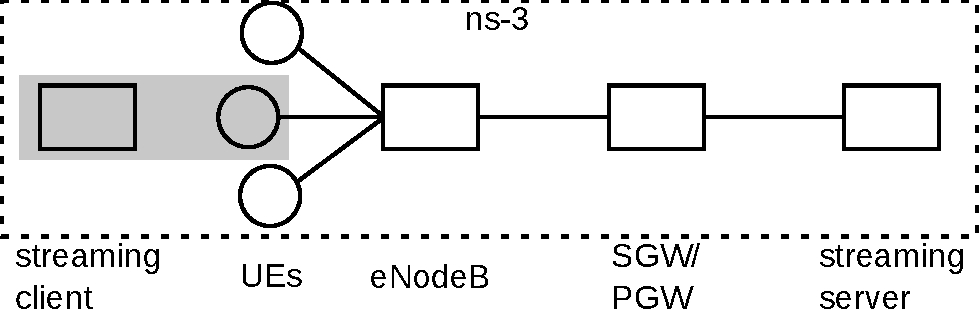
\includegraphics[width=0.6\textwidth]{images/streaming-simulation.pdf}
	\caption{\gls{LTE} reliable streaming simulation testbed.}
\label{c6:fig:streaming-simulation}
\end{figure}

The rest of the network model is kept as simple as possible as is visible in Figure~\ref{c6:fig:streaming-simulation}. LENA readily provides implementations for the \glspl{UE}, \gls{eNB}, and a combined \gls{SGW}/\gls{PGW} node. For the streaming simulation two things were added into this network. 

A node which acts as the storage server for the video segments was connected to the Internet-facing link of the \gls{PGW}. The storage server is kept as simple as possible. Upon receipt of a request for a specific segment over \gls{TCP} a dummy segment with the correct size is immediately sent to the client, reusing the open \gls{TCP} connection. %\todo{Segments typically have a size of ...?}
The gls{TCP} congestion avoidance mechanism implemented by ns-3 is New Reno, which also might not be ideally suited to mobile environments. Especially when compared to congestion avoidance mechanisms that are optimized for a high \gls{BDP} like Linux's CUBIC.

Note, the direct usage of \gls{TCP} instead of for example the more commonly used application layer protocol \gls{HTTP}. This should make no difference on the streaming process in the long run apart from the absence of a slight protocol overhead (i.e., the \gls{HTTP} headers) at the beginning of the transmission and for each segment. Using \gls{TCP} directly, however, simplifies the simulation and makes the results easier to interpret.

The client's playback buffering model is implemented as an application running on the \gls{UE}. The device also initiates the streaming and takes care of requesting each individual segment. However, the segments do not contain actual video data. Rather, the playback simulator just reads the list of frames and their size and synchronizes this information with the received amount of data to correctly calculate the buffer level.

During transmission, the \gls{LTE} framework sets up the lower layer protocols, which includes the radio stack and the \gls{gtp} core network bearer, accordingly. In the simplest model, only one \gls{eNB} and one \gls{UE} are present, to avoid interference with other devices. Moreover, a stationary mobility model with close distance to the transceiver is chosen. The model can be easily extended to factor in multiple devices and a mobility model with handover, all the capabilities are already present in ns-3. However, the simple setup was chosen to measure the upper limit of achievable performance. All of the other factors will undoubtedly reduce the performance. Otherwise, the \gls{LTE} nodes are left at their default configuration, which should yield an overall cell net bandwidth of \SI{80}{\mega\bit\per\second}

\begin{figure}[htb]
\centering
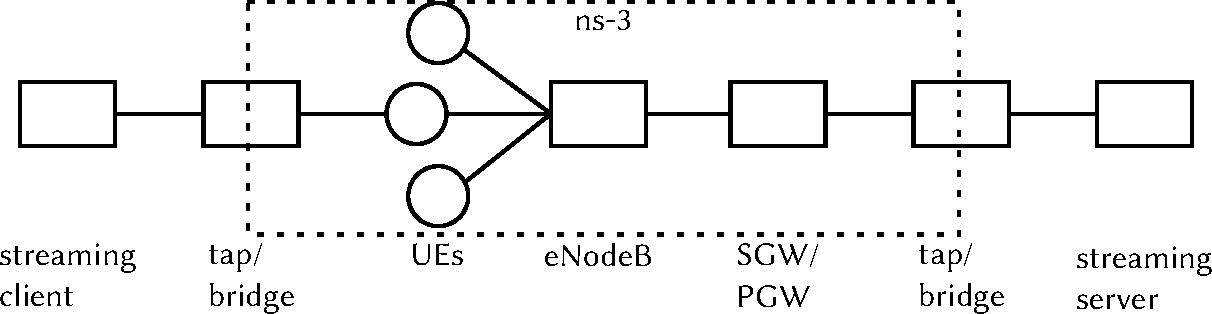
\includegraphics[width=1.0\textwidth]{images/streaming-hybrid.pdf}
\caption{Future testbed iteration: hybrid of ns-3 LTE simulation and actual or emulated streaming client and server bridged to it.}
\label{c6:fig:streaming-hybrid}
\end{figure}

Beyond its application as a pure simulation, a simulated ns-3 \gls{LTE} network could additionally be facilitated as a network emulator. Figure~\ref{c6:fig:streaming-hybrid} demonstrates such a setup. To be able to use it for a streaming emulation in the style of the measurements conducted in Section~\ref{c3:sec:measurements} a bridging device would need to be added on each side of the network, that interfaces with a real testbed network. The only effect of the simulated part is then to alter the \gls{QoS} parameters of the link according to its model. This approach is ideally suited to quickly test existing and already implemented streaming solutions for use with a mobile network and saves the effort of reimplementing them as a simulation model.


%%
\subsubsection{Simulated Streaming Models}

According to the classification and playback modeling from Sections~\ref{c3:sec:background} and \ref{c3:sec:model} the simulated model is a pull-based segmented video streaming system using \gls{TCP}. Two streaming models are suggested here, with the first suited for plain reliable streaming and the second modified to utilize the benefits of adaptive streaming.

Other playback models could be easily implemented as well, but these to should closely resemble the usual approaches taken by real reliable streaming players.


%%
\paragraph{Four Threshold Segmented Streaming Strategy}

This model is governed by four thresholds. They are, in the order of the buffer level they represent:

\begin{enumerate}
	\item \textit{Playback stop}. Represents the lower limit of the buffer and the player will stop if the level goes below this threshold. It can be set to as low as \SI{0}{\second} but it defaults to \SI{0.5}{\second} for this model. When the limit is underrun, stalling will occur.

	\item \textit{Transmission start}. If the transmission is currently stopped due to reaching the buffer limit, restart it if it falls beyond this threshold. Naturally, at the start of the streaming process segments are already requested at a buffer level of zero. The default is set to \SI{2.5}{\second} of video in the buffer. The gap to the playback stop threshold should be large enough to avoid stalls because of late transmission restarts.

	\item \textit{Playback start}. This threshold takes effect after every stalling event and restarts the player if at least this amount is in the buffer. It is set to \SI{5}{\second} here.

	\item \textit{Transmission stop}. In some scenarios this last threshold might not be necessary as it only acts to prevent a buffer overrun and lost video data. But most mobile devices suffer from rather low memory constraints and therefore need to limit the video buffer. When this limit is reached, no new segments are requested until the buffer falls below the transmission start limit again. It is set to \SI{10}{\second} here and is a soft limit that can be exceeded by still arriving segments. Therefore, it always needs to be set below the buffer's actual hard limit.
\end{enumerate}


\begin{figure}[htb]
	\centering
	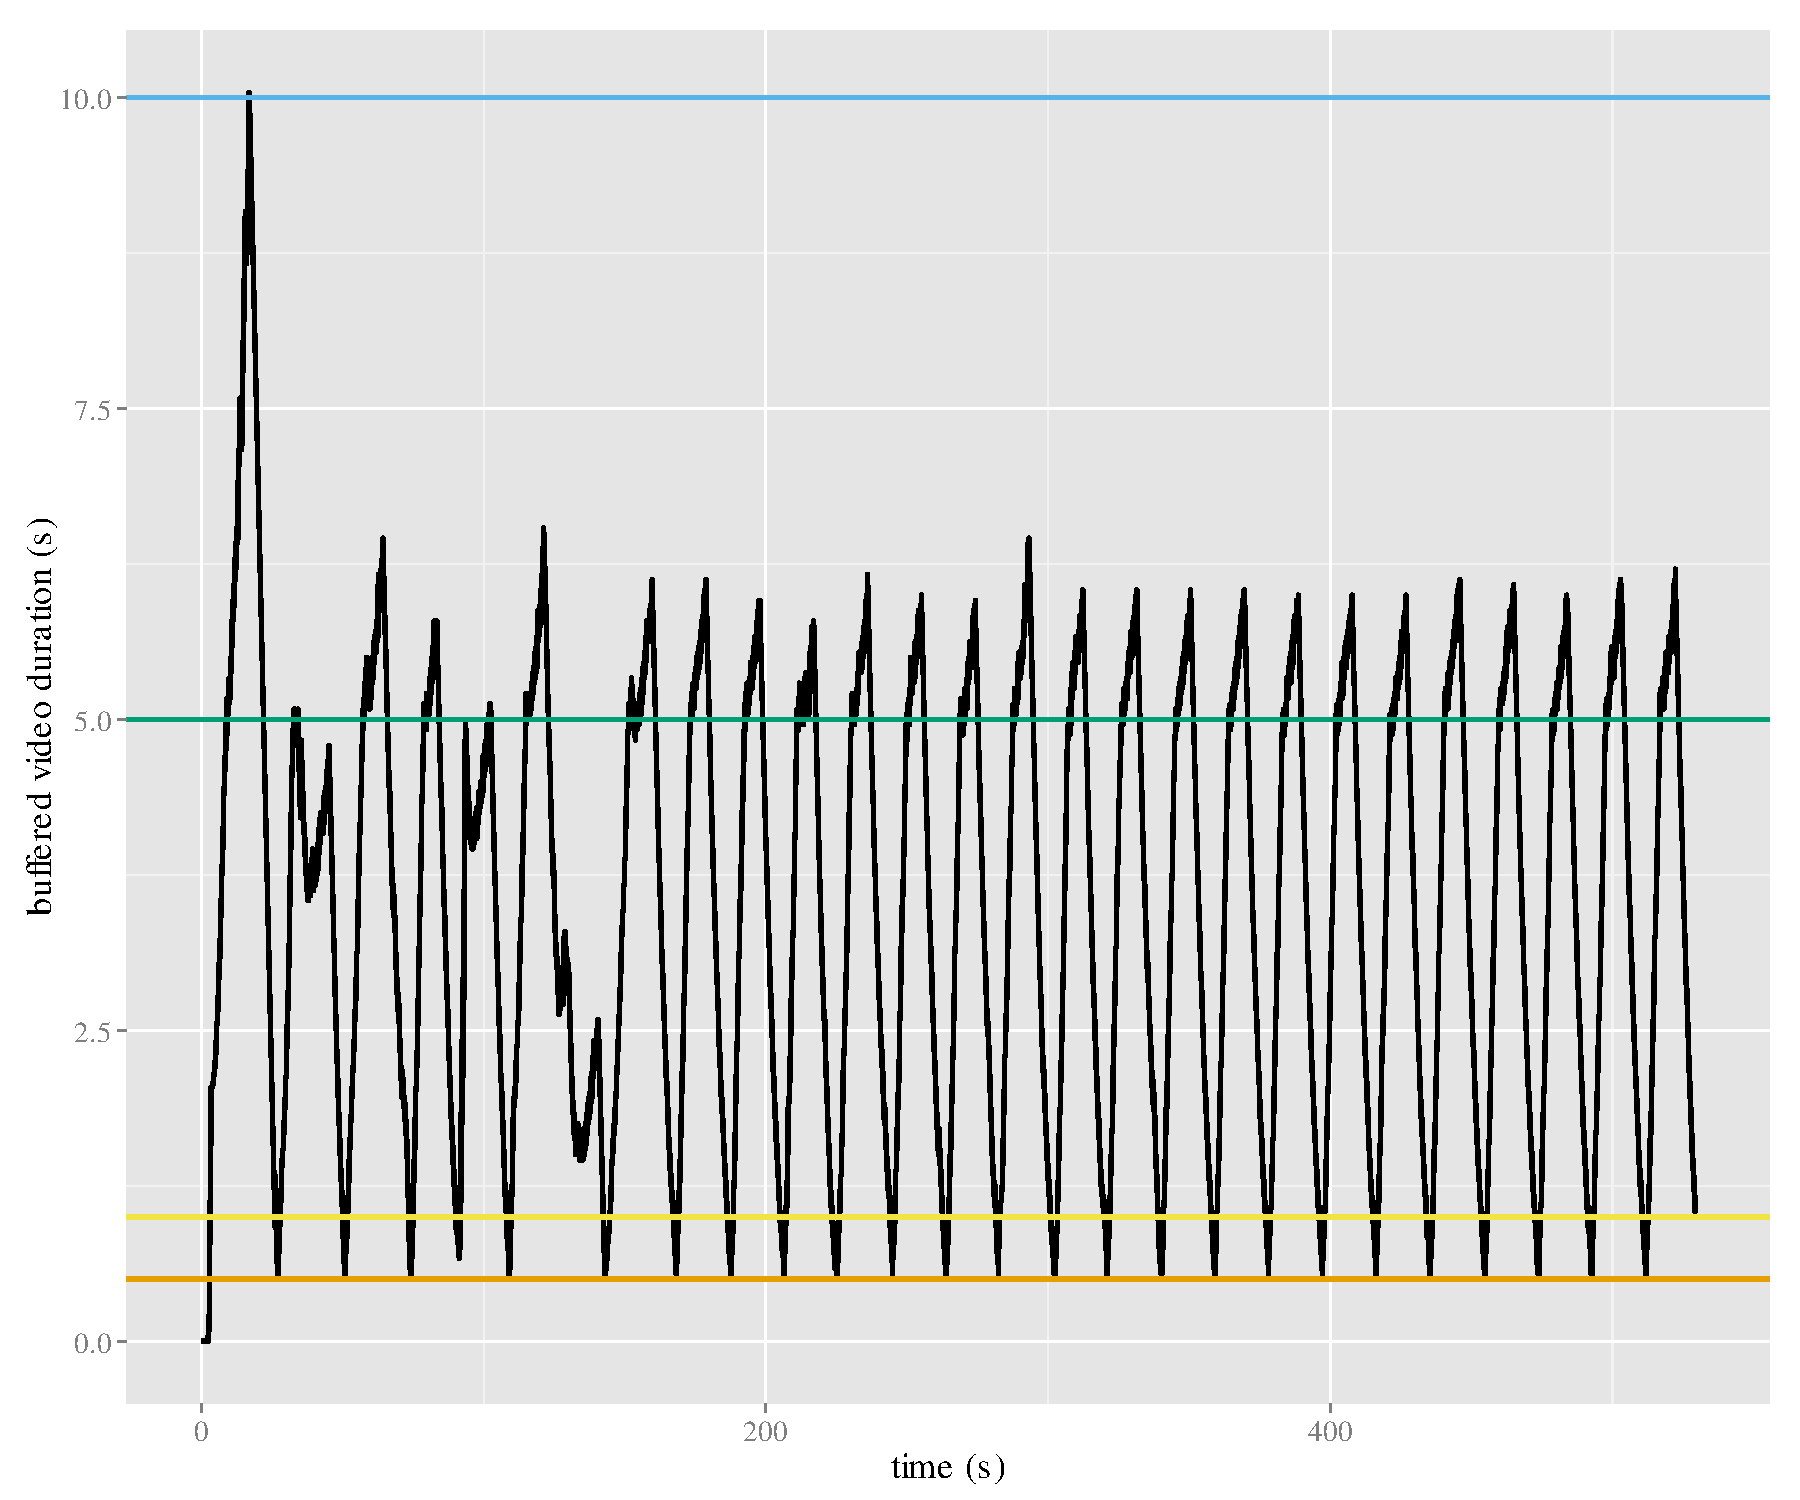
\includegraphics[width=0.9\textwidth]{images/R-ltesim-plotbuffer-time.pdf}
	\caption{Sample simulation run demonstrating the four threshold strategy.}
\label{c6:fig:ltesim-plotbuffer-time}
\end{figure}

To demonstrate the strategy an example scenario can be observed in Figure~\ref{c6:fig:ltesim-plotbuffer-time}. Depending on the relation of \gls{TCP} goodput to video bitrate a player with this strategy should always bounce between the thresholds 2 and 4 and never stop playing intermittently as in the example.

The default threshold values may be far from ideal and need to be optimized in the long run. But this is often the same case in real streaming solutions with the players arbitrarily preconfigured to values that could make sense from the developer's point of view without scientific validation.


%%
\paragraph{Six Threshold Window Scaling Adaptive Streaming Strategy}

By adding two additional thresholds the strategy could also be extended to work for adaptive reliable streaming. As a further prerequisite, all video segments need to be available in a number of quality levels and therefore video bitrates and seamless switching between levels at the segment borders needs to be possible. The more quality levels are present the better adaptable the streaming client can be, but it can work with as low as two levels. But this coarse switching between a very low number of levels will also be more noticeable by the user and might disturb her \gls{QoE} then a smooth decline in image quality.

The two new thresholds are values to trigger the switch to the next higher and lower segment quality level respectively. The reduce to lower quality threshold should be located between transmission start and playback stop, increase to higher quality situated between playback start and transmission stop. To accommodate more than two levels these two thresholds can be triggered multiple times. If the buffer level is still rising after the segment quality has been raised the quality should be raised again at the next opportunity. To better find a stable segment level candidate, the player should compute and keep track of the incline of the buffer level in the last time window. The steeper it gets the higher the chance for a quality level chance should be. The same rule applies also to the lower quality threshold.

While general quality changing support is present in the simulation model, this strategy is not fully implemented, but the basic four threshold strategy can be easily extended to match the adaptive strategy.


%%
\subsubsection{Scenario Evaluation}

To test the basic viability of the streaming simulation model (the \gls{LTE} model is taken as-is and covered by other research~\cite{Baldo:2013:OSM:2507924.2507940}) two test scenarios are defined and subsequently evaluated.

Common to both is the configuration of the video streaming simulation module. In both cases the simpler four threshold strategy is facilitated and tested with the three videos described in Table~\ref{c6:tbl:simulationvideos}.

Only one simulation run was conducted for each parameter setting as there are no known random factors involved that would merit running with different random seeds.

\begin{table}[htb]
	\caption{Test Video Parameters}
	\label{c6:tbl:simulationvideos}
	\centering
	\begin{tabu}{X[1.5,l]X[r]X[r,1.2]X[r]}
		\toprule
		\textbf{Parameter} & \textbf{Low Quality} & \textbf{Standard Quality} & \textbf{High Quality} \\
		\midrule
		Video Duration  & \SI{318}{\second} & \SI{602}{\second} & \SI{596}{\second} \\
		Size & \SI{19.2}{\mebi\byte} & \SI{258}{\mebi\byte} & \SI{853}{\mebi\byte}\\
		Frame rate & \SI{29.97}{\per\second} & \SI{29.97}{\per\second} & \SI{24}{\per\second}\\
		Average Video Bit rate & \SI{504}{\kilo\bit\per\second} & \SI{3596}{\kilo\bit\per\second} & \SI{12}{\mega\bit\per\second} \\
		Codec & H.263 & MPEG-4 & MPEG-4 \\
		\bottomrule
	\end{tabu}
\end{table}


%%
\paragraph{Congested Server Link}

This first series of evaluations exclusively looks at the \gls{QoS} of the streaming server's link and leaves the \gls{LTE} configuration unaltered.

The radio subsystem is configured to have a stationary \gls{UE} in close vicinity of the single \gls{eNB}. It should therefore reach the maximum attainable performance of radio link as it will be undisturbed by other users and fading effects. Therefore, it also represents the best case scenario for mobile streaming. If the streaming strategies and the associated video files reveal issues under these conditions they will surely also fail in an environment with a more degraded radio link.

The \gls{QoS} variables altered here are the link's bandwidth and delay. Loss will remain unchanged and at zero, as it will also result in just another source of delay for the reliable streaming process due to retransmission. 

Similar to the evaluations with the measurement framework of Section~\ref{c3:sec:measurements} no complex \gls{QoE} metrics will be computed. Rather, only the directly affected quality measures of a reliable streaming process will be observed: The total duration of the stalling phases in relation to the video's duration and the number of stalling phases.

\begin{figure}[htb]
	\centering
	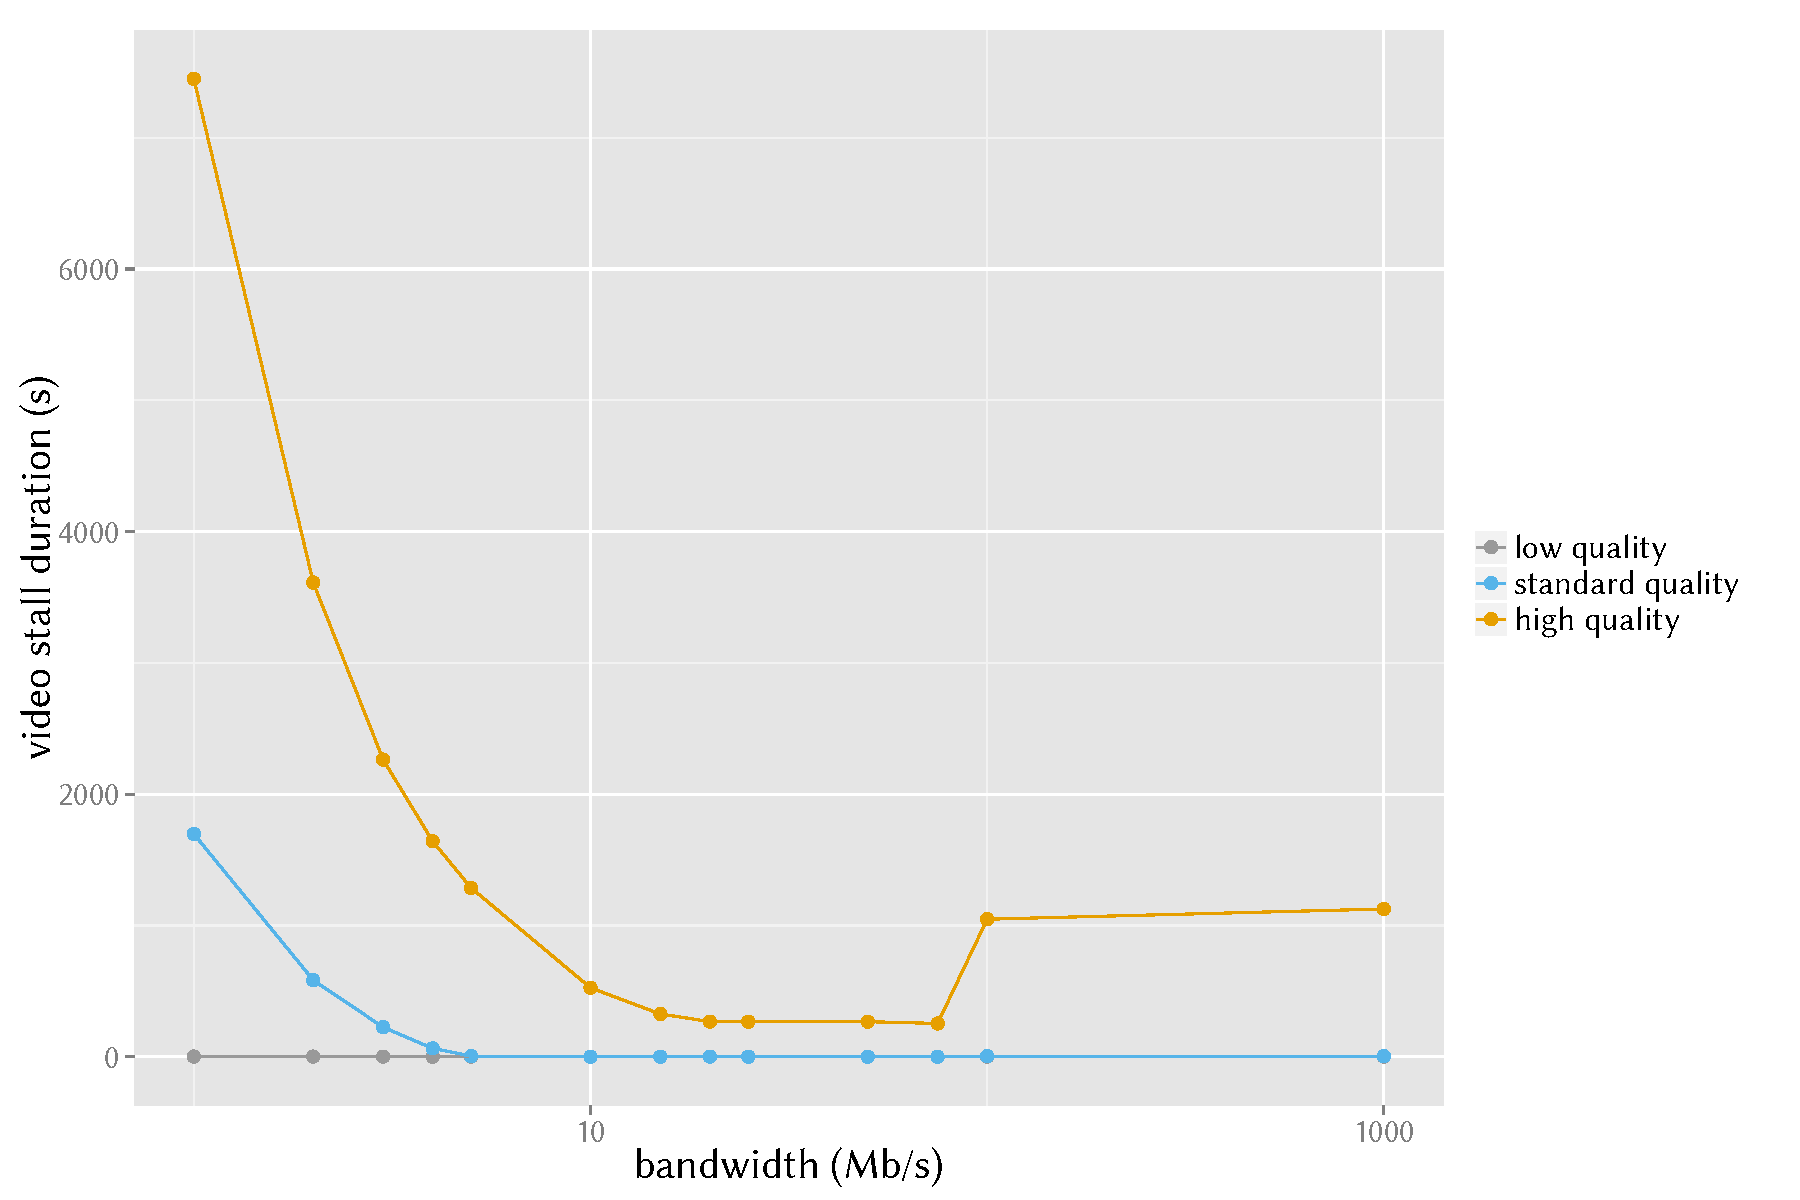
\includegraphics[width=0.9\textwidth]{images/R-ltesim-bwseries-stallduration.pdf}
	\caption{Relative stalling duration of the simulated reliable streaming player under limited Internet bandwidth.}
\label{c6:fig:ltesim-bwseries-stallduration}
\end{figure}

\begin{figure}[htb]
	\centering
	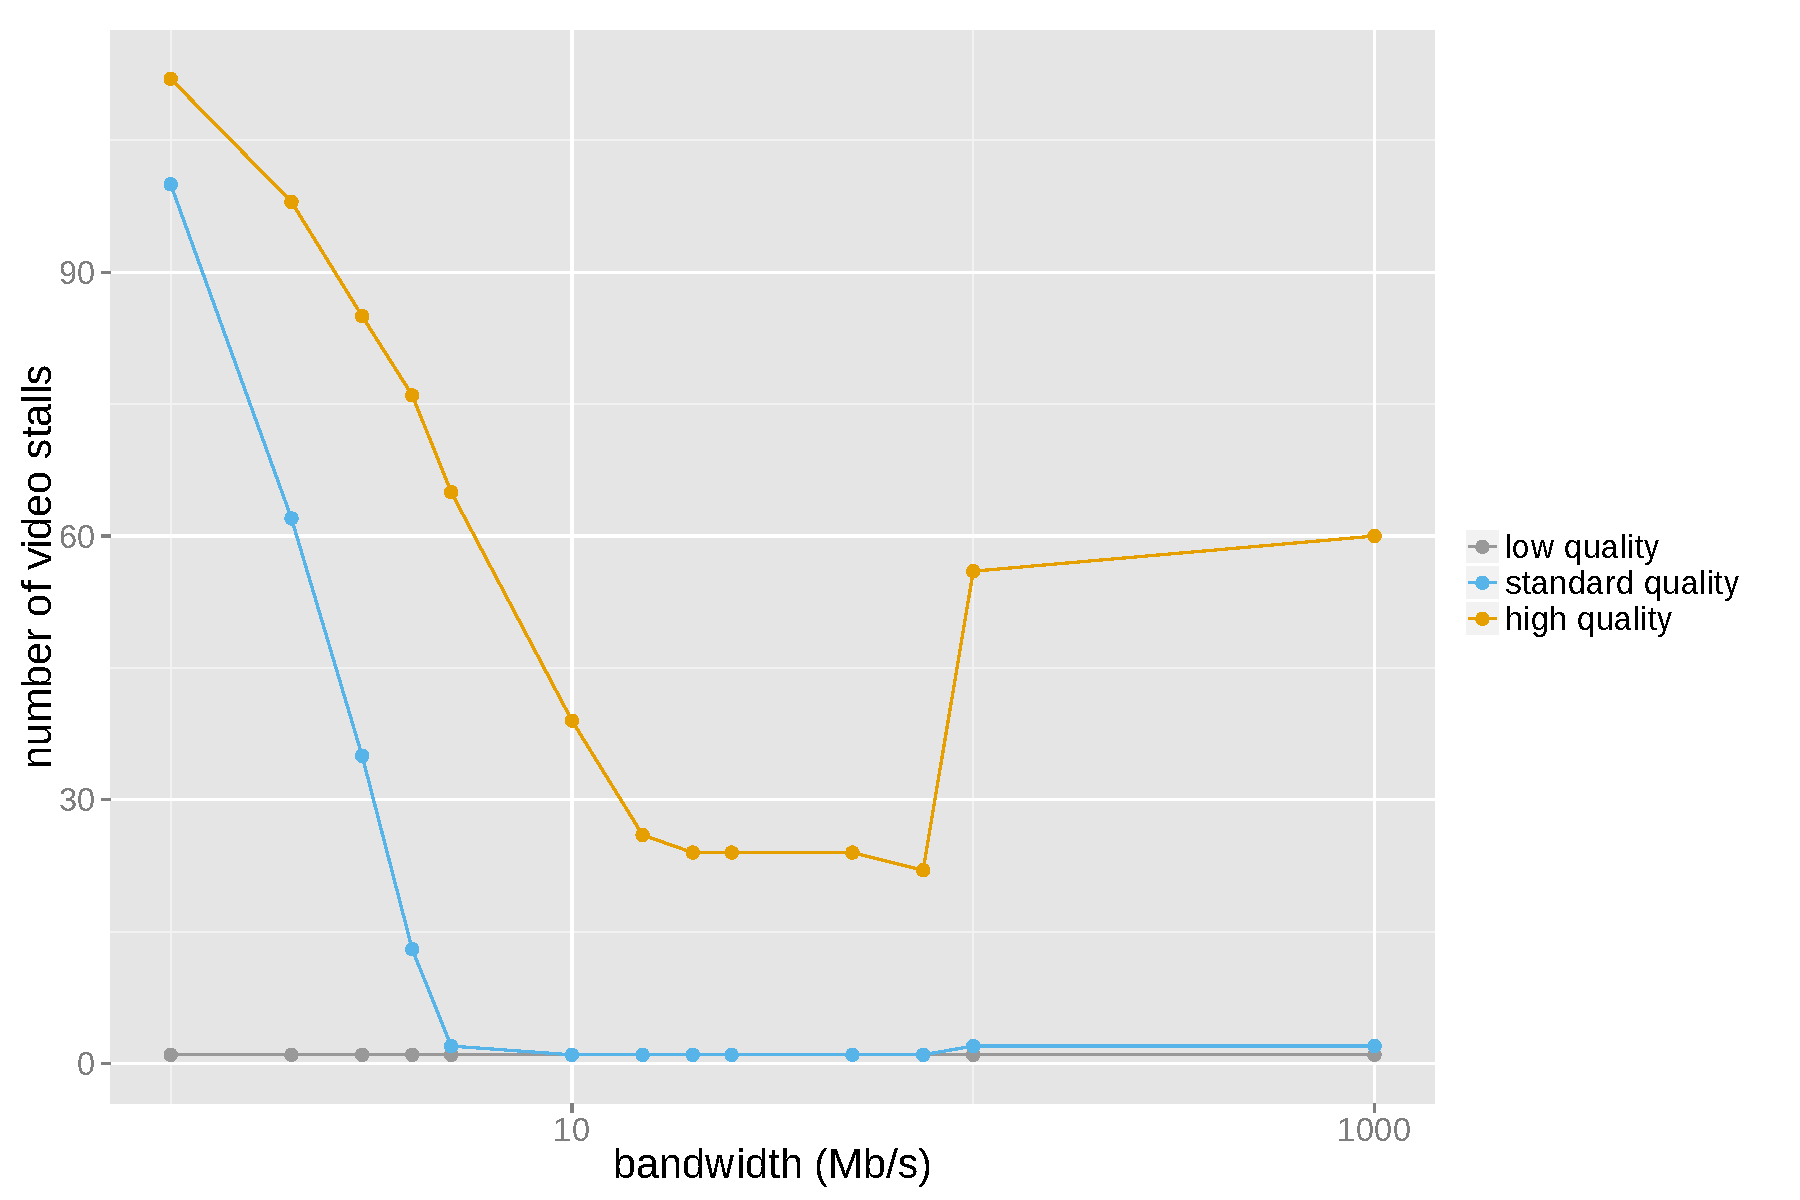
\includegraphics[width=0.9\textwidth]{images/R-ltesim-bwseries-numstalls.pdf}
	\caption{Number of stalling events of the simulated reliable streaming player under limited Internet bandwidth.}
\label{c6:fig:ltesim-bwseries-numstalls}
\end{figure}

The first series solely alters the bandwidth of the streaming server's link up to a maximum of \SI{1000}{\mega\bit\per\second}. The results are depicted in the Figures~\ref{c6:fig:ltesim-bwseries-stallduration} and \ref{c6:fig:ltesim-bwseries-numstalls}.

As soon as the link's bandwidth exceeds the video's bit rate, the number and duration of stalls are reduced. Stall events and duration in both the low and standard quality videos drop to zero. Only the high quality video does not show the same results. As its bit rate of \SI{12}{\mega\bit\per\second} should be perfectly manageable for the radio link some other explanation is required. 

A possible hypothesis are issues with the approach to requesting subsequent segments. As these need to be requested in a timely manner while other segments are still being transmitted, they could be requested to late and do not saturate the link anymore. 

However, this effect is somewhat contrary to the additional effect observed at link speeds of \SI{100}{\mega\bit\per\second} and above, where the stalling phases suddenly see an unexpected increase. As this happens exactly when the transmission speed exceeds the radio links capacity of about \SI{80}{\mega\bit\per\second} it might be an indication of the negative interaction of \gls{LTE}'s loss and congestion concealment with \gls{TCP}'s congestion avoidance mechanisms, related to the previously discussed bufferbloat issues. \gls{TCP} can not properly detect the bottleneck capacity in a timely manner as \gls{LTE} attempts to buffer and retransmit any packet exceeding the radio capacity below the user \gls{IP} layer. Through this issue, the effective goodput seems to get reduced to about \SI{5}{\mega\bit\per\second}, which is not enough for the high quality video to stream without interruption.

%\todo{check pcaps for >=100mbit experiments; could also be related to issues of the actual lte simulation network but implementation can not fully responsible for this?}

\begin{figure}[htb]
	\centering
	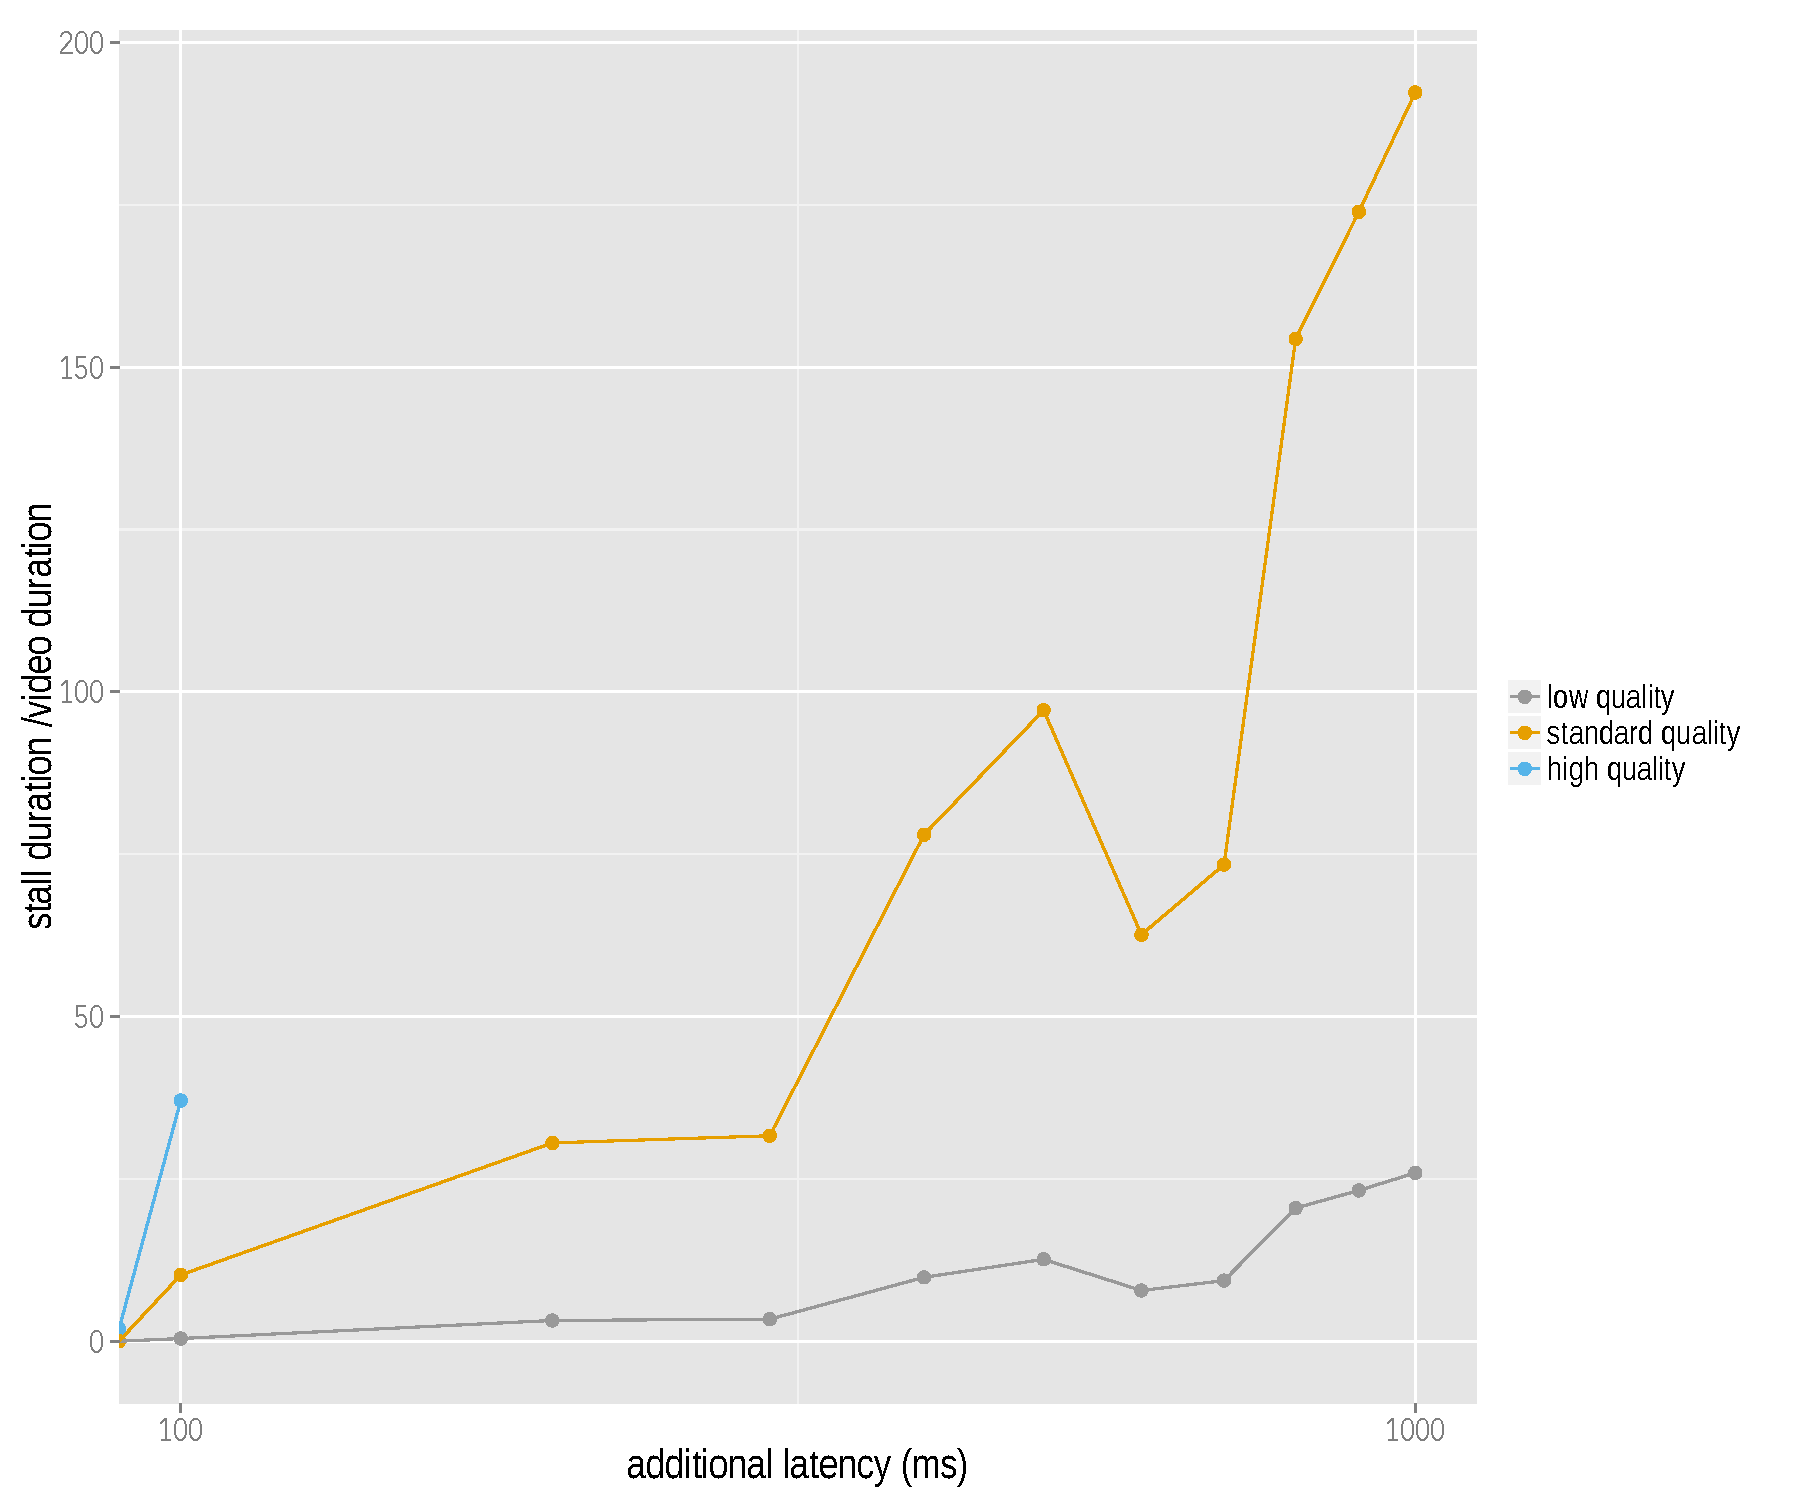
\includegraphics[width=0.9\textwidth]{images/R-ltesim-latencyseries-stallduration.pdf}
	\caption{Relative stalling duration of the simulated reliable streaming player under increased Internet latency.}
\label{c6:fig:ltesim-latencyseries-stallduration}
\end{figure}

\begin{figure}[htb]
	\centering
	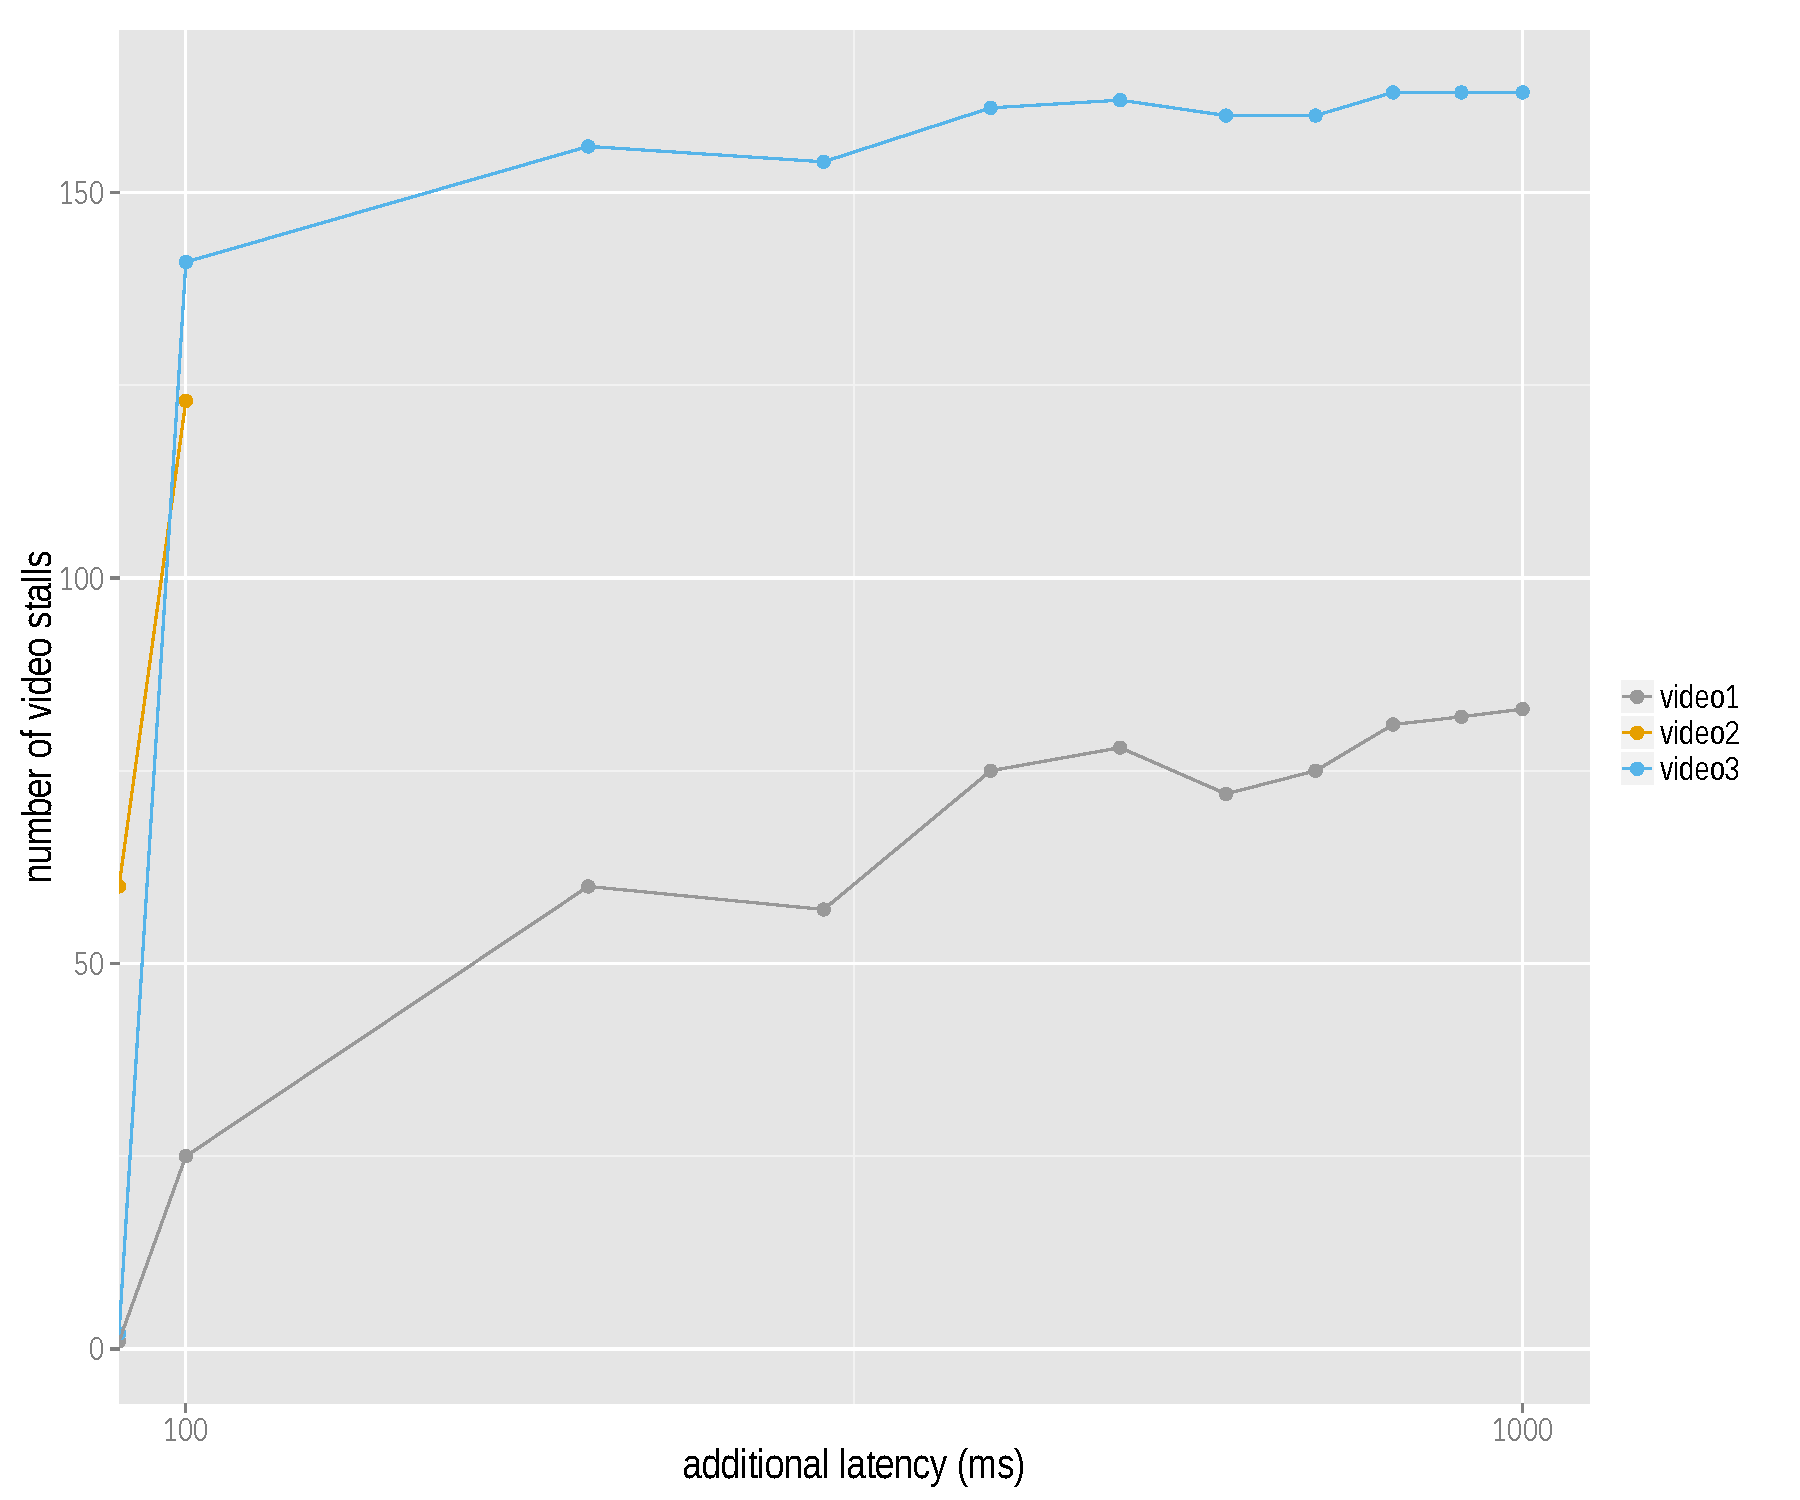
\includegraphics[width=0.9\textwidth]{images/R-ltesim-latencyseries-numstalls.pdf}
	\caption{Number of stalling events of the simulated reliable streaming player under increased Internet latency.}
\label{c6:fig:ltesim-latencyseries-numstalls}
\end{figure}

In a second series of simulation runs the latency of the server's link was increased incrementally up to an additional latency of \SI{1000}{\milli\second}. The values were set deterministically with no probability distribution. Figures~\ref{c6:fig:ltesim-latencyseries-stallduration} and \ref{c6:fig:ltesim-latencyseries-numstalls} again show the results in terms of the relative duration and number of stalling phases. The playback simulation seems to be excessively sensitive to latency increases. Even a small \SI{100}{\milli\second} increase makes the high and standard quality videos completely unwatchable as the stalling duration is more than ten times longer than the actual video. With latencies beyond \SI{100}{\milli\second} the high quality video could not be successfully streamed anymore. 


This behavior can partially be attributed to the simplistic segment request strategy used in this experiment. New segment are only requested when the previous one has fully arrived. As this takes a full round trip, the latency has a significant influence on the arrival time of subsequent segments. To avoid this kind of stop-and-wait behavior in the segment request process, new segments need to be requested sufficiently in advance while the previous segment is still being transmitted, so that the full bandwidth is always utilized.

With these improvements to the retrieval strategy this specific issue can be eliminated. But this just shows the many pitfalls and influences of various layers. A simple implementation detail may have large implications on the streaming quality the user experience.


%%
\paragraph{Device Mobility}

\begin{figure}[htb]
	\centering
	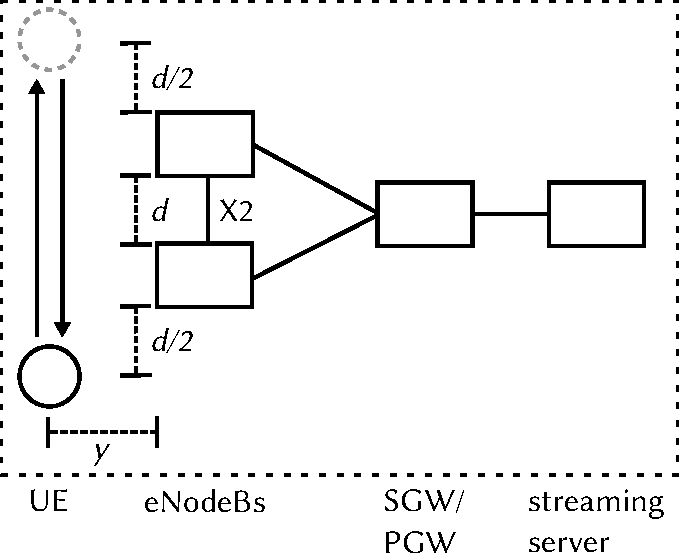
\includegraphics[width=0.5\textwidth]{images/streaming-simulation-mobility.pdf}
	\caption{Simulated handover mobility scenario using waypoints.}
\label{c6:fig:streaming-simulation-mobility}
\end{figure}

Besides altering the server link, the effects of the simulated \gls{LTE} network can also be investigated through various means. Here, mobility will be under scrutiny. For this, a second \gls{eNB} will be added to the network. Both are connected through the X2 interface, which will be used for the \gls{eNB}-anchored mobility provided by LENA. Instead of having a constant position relative to the \gls{eNB}, the \gls{UE} will no move back and forth between two waypoints on a two-dimensional plane in parallel to the two base stations which are placed at a distance of $d$ between each other. A handover is triggered each time the device leaves the range of one station and enters the other. Furthermore, the horizontal distance on the 2D-plane between the device and the \glspl{eNB} is controlled by a second parameter $y$. Figure~\ref{c6:fig:streaming-simulation-mobility} depicts this scenario and the positioning of the waypoints.

\begin{figure}[htb]
	\centering
	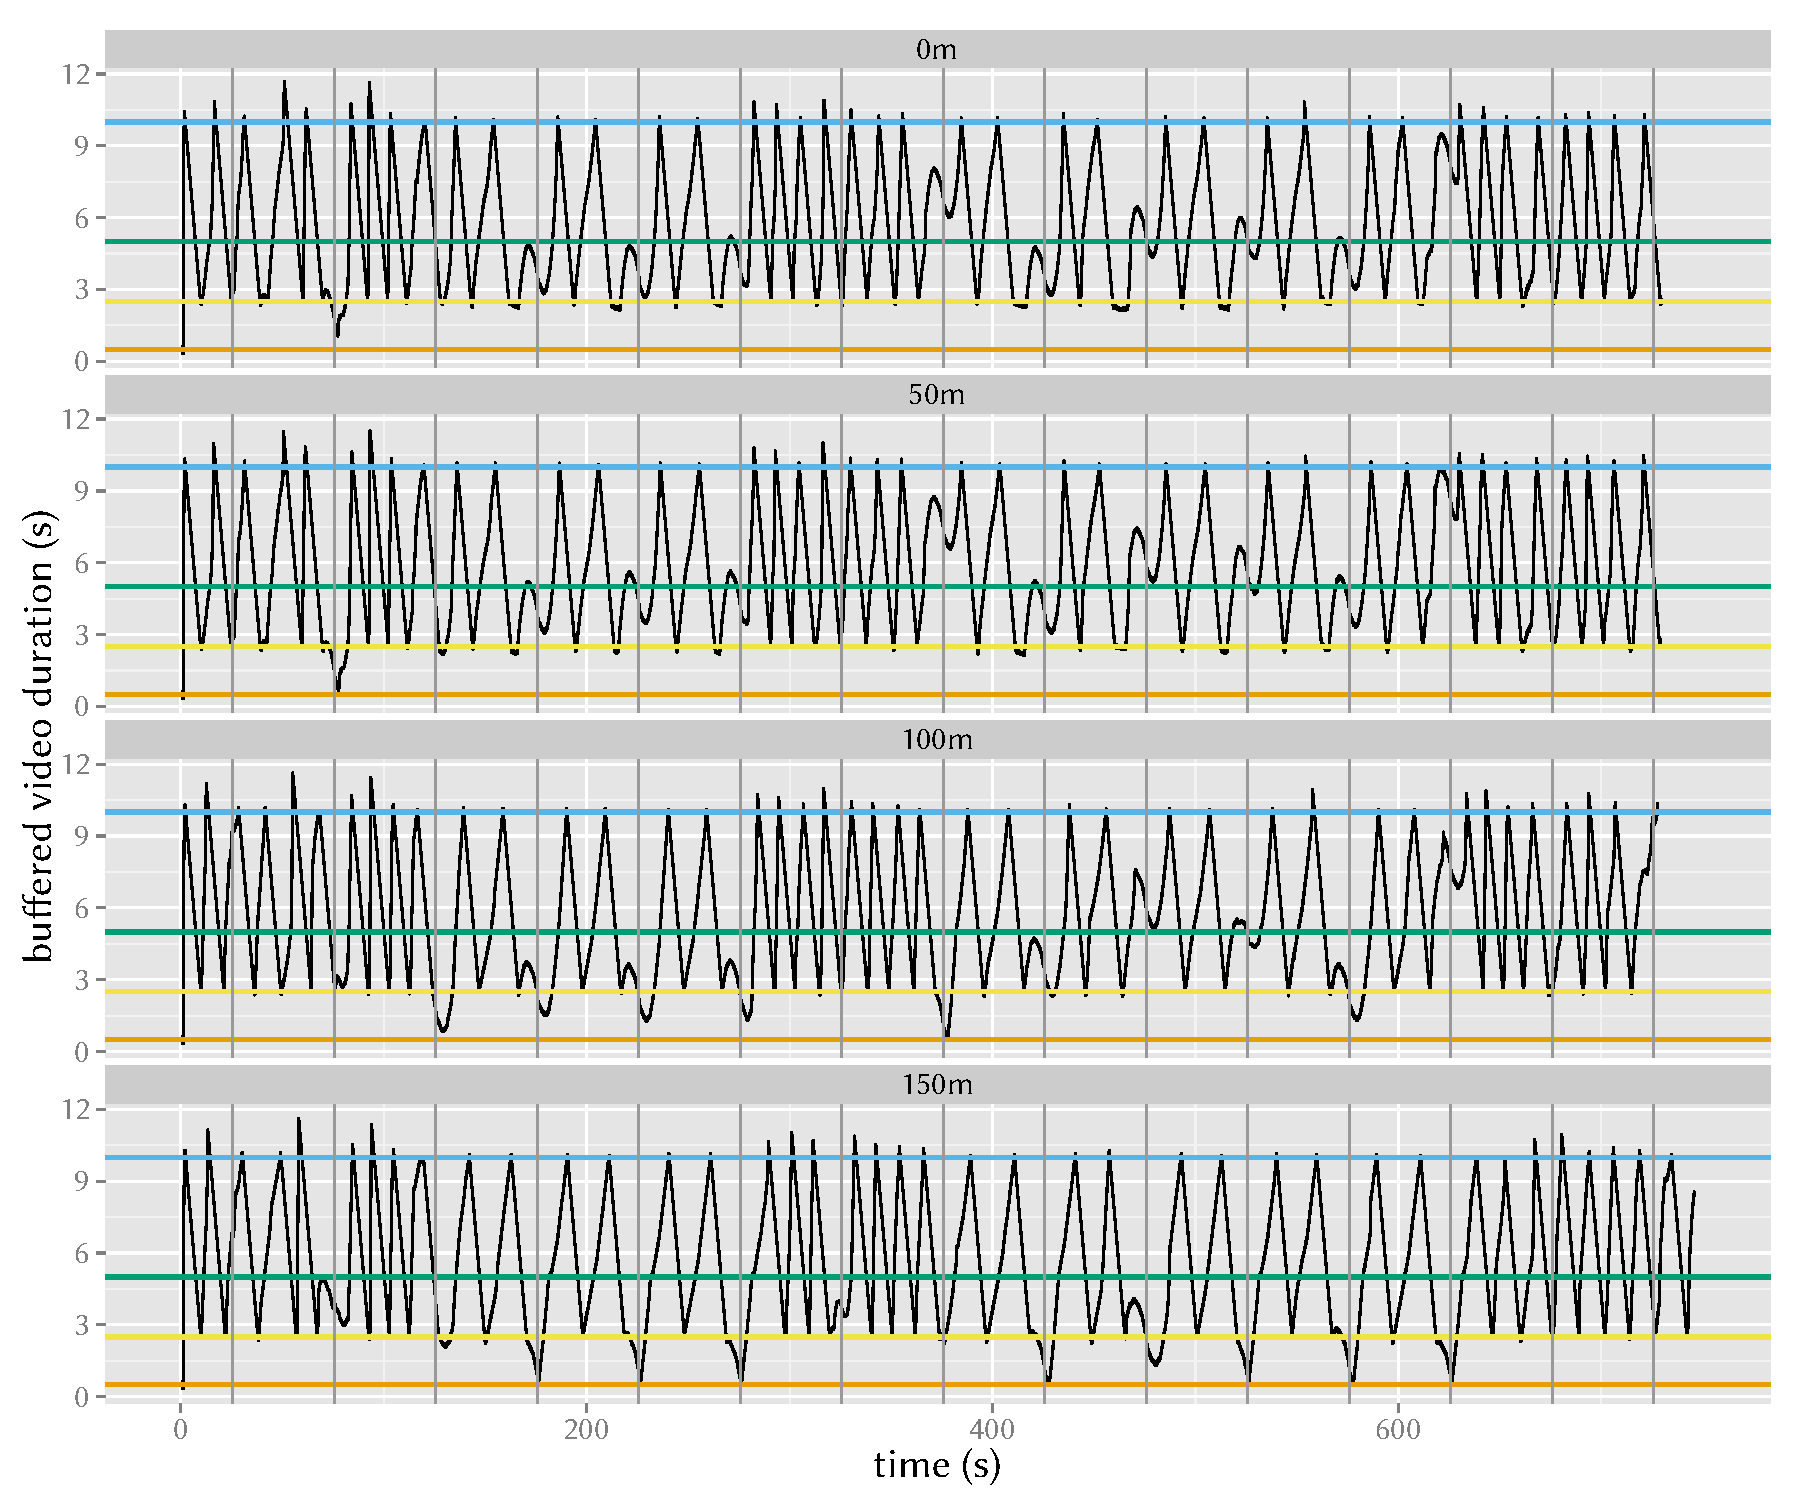
\includegraphics[width=0.9\textwidth]{images/R-ltesim-plotbuffer-mobility-facets.pdf}
	\caption{Playback buffer time series of the simulated mobility experiments with increasing distance between device and \glspl{eNB}.}
\label{c6:fig:ltesim-mobility-plotbuffer-facets}
\end{figure}

For the purpose of this experiment, the two \glspl{eNB} were placed at a vertical distance of $d=\SI{500}{\meter}$ while the horizontal distance to the device was varied between $y=\SI{0}{\meter}$ and $y=\SI{150}{\meter}$. The device is moving at a constant velocity of \SI{20}{\meter\per\second}. During the movement the standard quality video was streamed to the device and its playback simulated. 

The results in terms of the buffer fill level are displayed in Figure~\ref{c6:fig:ltesim-mobility-plotbuffer-facets}. The color-coded horizontal lines once again demark the same thresholds from the previously described four threshold segmented streaming strategy.

The handover events between the two \gls{eNB} are denoted by the gray vertical lines. The actual control transfer usually last for only about \SI{40}{\milli\second}. But looking at the figures it is immediately evident that the video buffer, and therefore the throughput of the video segments, already suffers seconds before this handover event when the edge of the radio range of the currently active \gls{eNB} is reached. The playback stop threshold is undercut several times right at the handover mark and stalling occurs.

It seems, that the throughput at the radio edge drops below the video's average bitrate of \SI{3596}{\kilo\bit\per\second}. Therefore, the buffer cannot be maintained for this quality. If the buffer was at a low level beforehand, it will run empty and lead to stalling due to the mobility. Additionally, there seems to be a dependence of the stalling probability on the distance between device and base station. A farther distance decreases the achievable throughput leading to an increased chance of the buffer running empty.

Mobile streaming playback strategies can attempt to counteract mobility-related issues in a number of ways. A simple approach would be to adjust the threshold levels to allow for a much larger buffer while also restarting transmissions earlier. But this comes at the price of an increased memory resource usage on the device, which might not possible in every scenario. Second, the strategy can be exchanged for an adaptive one, for example the described six threshold window scaling strategy with appropriately chosen threshold values. Here, the stalls are exchanged for phases of lower quality video, which can be acceptable under circumstances. 

Finally, both non-adaptive and adaptive strategies can be improved by employing the cross-layer model described in Section~\ref{c5:sec:crosslayerhinting}. By utilizing information from the radio network layers, handover events can be detected sufficiently in advance and an appropriate reaction chosen by the playback strategy. For example by temporarily increasing the maximum buffer threshold and requesting segments more rapidly or by quickly dropping to a lower quality level and filling the buffer up.

%%
\paragraph{Further Scenarios}

Apart from the experiments conducted here, some others are also worth investigating but out of scope for this work.

If one plans to implement a reliable streaming solution, the simulation can be utilized to test any kind of playback strategy and transmission mechanics and attune it to mobile networks. 

Besides developing entirely new playback strategies, the default thresholds of the four and six threshold strategies should also be optimized through iterative simulation of value combinations.

The opposite approach would also be possible for mobile network operators: Map the operator's mobile network infrastructure onto the simulation and test the performance of existing streaming strategies with it. If any issues or performance bottlenecks are discovered, the operator can make adjustments to the infrastructure and implement these changes afterwards outside of the simulation.

It would also be worthwhile to see the impact of the cross-layer model described in Section~\ref{c5:sec:crosslayerhinting} as they are specifically intended to reduce the influence this kind of mobile network architecture has on user applications. An implementation of cross-layer hinting would be relatively simple here, as the layer isolation boundaries are much easier to circumvent in a network simulator.

As mentioned earlier, ns-3's \gls{LTE} framework does only implemented a limited subset of the \gls{3GPP} specifications, mainly related to the user plane and the radio link stack. Almost no control plane procedures are implemented. This may have only a negligible impact as soon as a connection is established and remains stable and only a very small number of users are connected to the system. But this is not the norm for an actual mobile network in operation with its mobility features and high churn, both in terms of data flows as well as mobile users, generating a large amount of signaling traffic as was discussed before in Section~\ref{c4:sec:3gpparchitecture}. To best mimic the dataset evaluations related to \gls{PDP} context and \gls{gtp} tunnel life cycle management conducted in Section~\ref{c4:sec:evaluations}, the simulator would need to at least be able to reproduce these tunnel management and the related \gls{RRC} \gls{PDP} context procedures happening on the user traffic path. Therefore, it is worth to reconduct the above experiments as soon as the framework has made any progress in this direction.




% \url{http://www.valid8.com/UMTS_Core_Network_Simulator.html} Not publicly available and commercial
% also seems to focus on the circuit switched domain


% Only commercial: UMTS model in OPNET (which was renamed to Riverbed Modeler)\footnote{\url{http://www.riverbed.com/products/performance-management-control/network-performance-management/network-simulation.html}} 
% again radio and user plane focused

%\url{http://www.nsnam.org/docs/release/3.20/doxygen/group__lte.html}
%\url{http://www.nsnam.org/docs/release/3.20/models/html/lte.html}

%Reasoning why ns-3/LENA will be used here.
%but combined with ns-3 offers almost complete representation of a vanilla network and transport level network stack


%performance: eNB has 25 resource block each up/down; suggests 5Mhz BW
%https://groups.google.com/forum/#!searchin/ns-3-users/lte/ns-3-users/dwMjWwJBdBw/wfWCcRctN4EJ



% LQ
% MP4 container
% 352x288
% AAC audio, 11KHz
% \SI{24.0}{\kilo\bit\per\second} audio bitrate)
% \SI{531.0}{\kilo\bit\per\second} overall bitrate
% SD
% DivX container
% 720x400
% MP3 audio, 44.1Khz
% \SI{128}{\kilo\bit\per\second} audio bitrate
% \SI{3735}{\kilo\bit\per\second} overall bitrate
% HQ
% AVI container
% 1920x1080
% AC-3 audio, 48Khz
% \SI{448}{\kilo\bit\per\second} audio bitrate
% \SI{12.5}{\mega\bit\per\second} overall bitrate